%%%%%%%%%%%%%%%%%%%%%%%%%%%%%%%%%%%%%%%%%
% Engineering Calculation Paper
% LaTeX Template
% Version 1.0 (20/1/13)
%
% This template has been downloaded from:
% http://www.LaTeXTemplates.com
%
% Original author:
% Dmitry Volynkin (dim_voly@yahoo.com.au)
%
% License:
% CC BY-NC-SA 3.0 (http://creativecommons.org/licenses/by-nc-sa/3.0/)
%
%%%%%%%%%%%%%%%%%%%%%%%%%%%%%%%%%%%%%%%%%

%----------------------------------------------------------------------------------------
%	PACKAGES AND OTHER DOCUMENT CONFIGURATIONS
%----------------------------------------------------------------------------------------

\documentclass[12pt,a4paper]{article} % Use A4 paper with a 12pt font size - different paper sizes will require manual recalculation of page margins and border positions
\usepackage[utf8]{inputenc}
\usepackage{marginnote} % Required for margin notes
\usepackage{wallpaper} % Required to set each page to have a background
\usepackage{lastpage} % Required to print the total number of pages
\usepackage[left=1.3cm,right=1.3cm,top=1.8cm,bottom=2.2cm,marginparwidth=3.4cm]{geometry} % Adjust page margins
\usepackage[fleqn]{amsmath} % Required for equation customization
\usepackage{amssymb} % Required to include mathematical symbols
\usepackage{xcolor} % Required to specify colors by name
\usepackage{xfrac}
\usepackage{fancyhdr} % Required to customize headers
\usepackage{booktabs}
\usepackage{xargs}
\usepackage{mathtools}
\usepackage{multirow}
\usepackage{graphicx}
\usepackage{lipsum}
\usepackage{enumitem}
\usepackage[linewidth=0.5pt]{mdframed}

\graphicspath{ {images/} }
\setlength{\headheight}{12mm} % Increase the size of the header to accommodate meta-information
\pagestyle{fancy}\fancyhf{} % Use the custom header specified below
\renewcommand{\headrulewidth}{0pt} % Remove the default horizontal rule under the header

\setlength{\parindent}{0cm} % Remove paragraph indentation
\newcommand{\tab}{\hspace*{2em}} % Defines a new command for some horizontal space

\newcommand\BackgroundStructure{ % Command to specify the background of each page
	\setlength{\unitlength}{1mm} % Set the unit length to millimeters

	\setlength\fboxsep{0mm} % Adjusts the distance between the frameboxes and the borderlines
	\setlength\fboxrule{0.25mm} % Increase the thickness of the border line
	%%\put(10, 15){\fcolorbox{black}{white!10}{\framebox(150,260){}}} % Main content box
	%%\put(150, 15){\fcolorbox{black}{gray!10}{\framebox(45,260){}}} % Margin box
%%	\put(10, 278){\fcolorbox{black}{white!10}{\framebox(192, 12){}}} % Header box
%% \put(137, 263){\includegraphics[height=23mm,keepaspectratio]{logo}} % Logo box - maximum height/width: 
}
\newcommand\const{\mathrm{const}}
\newcommand\solve[2]{\text{solve}\left\(#1\;\text{pour}\;#2\right\)}
%% \newcommand\vec\overrightarrow

\newcommand\textsup[1]{\ensuremath{^{\textrm{#1}}}}
\newcommand\textsub[1]{\ensuremath{_{\textrm{#1}}}}

\newcommand\frametitle[1]{ {\bfseries #1} \\[5pt] }
\newcommand\framenote[1]{
	{\small {\bfseries notes} \\ #1}
}
\newcommand\integrate[2][x]{\int #2 \,\mathrm{d}#1}
\newcommand\integratediff[4][x]{\int_{#2}^{#3} #4 \,\mathrm{d}#1}

%----------------------------------------------------------------------------------------
%	HEADER INFORMATION
%----------------------------------------------------------------------------------------

\fancyhead[L]{
	{\LARGE Formulaire de physique}
}
\fancyfoot[R]{
	{\small \thepage/\pageref{LastPage}}
}


%----------------------------------------------------------------------------------------

\begin{document}

\newenvironmentx{twocols}[3][1=0.5, 2=0.4, 3=c]{
	\def\colonewidth{#1}
	\def\coltwowidth{#2}
	\def\mpagealign{#3}
	\providecommand\nextcol{
		%%\vspace{0.4em}
		\end{minipage}
		\vrule\quad
		\begin{minipage}[\mpagealign]{\coltwowidth\textwidth}
		%%\vspace{0.4em}
	}
	\begin{minipage}[\mpagealign]{\colonewidth\textwidth}
	%%\vspace{0.4em}
}{
	%%\vspace{0.4em}
	\end{minipage}
}
\newenvironmentx{vardef}{
	\renewcommand\item[2]{ {##1} & {##2} \\ }
	\begin{tabular}{rl}
}{
	\end{tabular}
}

\AddToShipoutPicture{\BackgroundStructure} % Set the background of each page to that specified above in the header information section

%----------------------------------------------------------------------------------------
%	DOCUMENT CONTENT
%----------------------------------------------------------------------------------------

\section{Mouvements}

\subsection{Mouvement Rectiligne}
Mouvement d'un corps sur une trajéctoire réctiligne.
\subsubsection*{Uniforme (MRU)}
\begin{twocols}[0.5][0.5]
	\[
	\left\{
		\begin{aligned}
			v &= \const \\
			x &= x_0 + v \cdot t \\
		\end{aligned}
	\right.
	\]
\nextcol
	\begin{vardef}
		\item{$v$}{Vitesse [$m/s$]}
		\item{$x$}{Position [$m$]}
		\item{$x_0$}{Position initiale [$m$]}
		\item{$t$}{Temps [$s$]}
	\end{vardef}
\end{twocols}
\subsubsection*{Uniformément Accéléré (MRUA)}
\begin{twocols}
	\[
	\left\{
		\begin{aligned}
			a &= \const \\
			v(t) &= v_0 + a \cdot t \\
			x(t) &= x_0 + v_0 \cdot t + \frac{a \cdot t^2}{2} \\
		\end{aligned}
	\right.
	\]
\nextcol
	\begin{vardef}
		\item{$a$}{Accélération [$m/s^2$]}
		\item{$v_0$}{Vitesse initiale [$m/s$]}
	\end{vardef}
\end{twocols}

\subsection{Mouvement Circulaire}
Mouvement d'un corps autour d'un point de rotation (trajectoire circulaire).
\subsubsection*{Uniforme (MCU)}
\begin{twocols}[0.5][0.5]
	\[
	\left\{
		\begin{aligned}
			\omega &= \const \\
			\omega &= \frac{\Delta\theta}{\Delta t} \\
			\theta &= \omega \cdot t + \theta_0 \\
		\end{aligned}
	\right.
	\]
\nextcol
	\begin{vardef}
		\item{$\omega$}{Vitesse angulaire [$rad/s$]}
		\item{$\theta$}{Angle [$rad$]}
		\item{$\theta_0$}{Angle initial [$rad$]}
		\item{$t$}{Temps [$s$]}
	\end{vardef}
\end{twocols}
\subsubsection*{Uniformément Accéléré (MCUA)}
\begin{twocols}
	\[
	\left\{
		\begin{aligned}
			\alpha &= \const \\
			\omega &= \omega_0 + \alpha \cdot t \\
			\theta &= \theta_0 + \omega \cdot t + \frac{\alpha \cdot t^2}{2} \\
			V &= \omega \cdot r \\
			a_c &= \frac{V^2}{r}\;\text{OU}\;\omega^2 \cdot r \\
			F_c &= m \cdot a_c \\
		\end{aligned}
	\right.
	\]
\nextcol
	\begin{vardef}
		\item{$r$}{Rayon [m]}
		\item{$\alpha$}{Accélération angulaire [$rad/s^2$]}
		\item{$\omega_0$}{Vitesse angulaire initiale [$rad/s$]}
		\item{$V$}{Vitesse tangantielle [$m/s$]}
		\item{$a_c$}{Accélération centripète [$m/s^2$]}
		\item{$F_c$}{Force centripète [$N$]}
	\end{vardef}
\end{twocols}

\newpage

\section{Balistique}

\begin{figure*}[h]
	\centering
	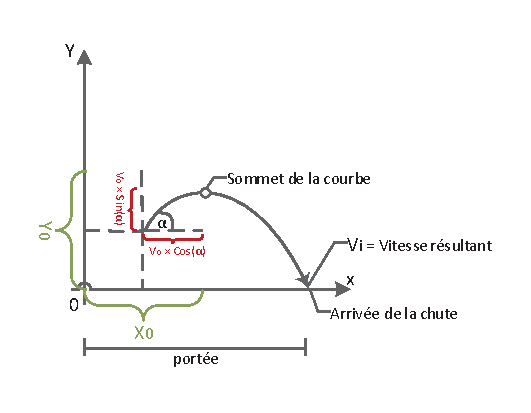
\includegraphics{Balistique}
\end{figure*}
\emph{Au sommet de la courbe: $v_y(t) = 0$}

\subsection{Equations du mouvement}
\begin{twocols}[0.5][0.5]
	Acceleration
	\begin{equation*}
	\left\{
		\begin{aligned}
			a_x &= 0 \\
			a_y &= -g \\
		\end{aligned}
	\right.
	\end{equation*}
	\par\vspace{1em}
	Vitesse
	\begin{equation*}
	\left\{
		\begin{aligned}
			v_x(t) &= v_0 \cdot \cos{\alpha} \\
			v_y(t) &= v_0 \cdot \sin{\alpha}+a_y \cdot t \\
		\end{aligned}
	\right.
	\end{equation*}
\nextcol

	Position
	\begin{equation*}
	\left\{
		\begin{aligned}
			x(t) &= x_0+v_0 \cdot \cos{\alpha} \cdot t \\
			y(t) &= y_0+v_0 \cdot \sin{\alpha} \cdot t+{\displaystyle\frac{a \cdot t^2}{2}} \\
		\end{aligned}
	\right.
	\end{equation*}

\end{twocols}

\subsection*{Equations annexes}
\emph{A utiliser avec précautions, ne s'appliquent pas dans tous les cas.}
\par\vspace{1em}
\begin{twocols}[0.5][0.4][t]
	Port\'ee
	\begin{equation*}
		\left\{
		\begin{array}{rll}
			p &= {\displaystyle \frac{v_0\,^2 \cdot \sin (2 \cdot \alpha)}{a_y}} & \text{Si}\:y_0 = 0 \\[1em]
			p &= \text{résoudre}\:\left\{
					\begin{aligned}
						y(t) &= 0 \\
						x(t) &= n \\
					\end{aligned}
			\right.
				\text{pour} \: n
			 & \text{Si}\:y_0 \neq 0
		\end{array}
		\right.
	\end{equation*}

\nextcol

	Alt. Maximale
	\begin{equation*}
		y_\text{max} = \frac{(v_0\cdot\sin{\alpha})^2}{2 \cdot a_y} + y_0
	\end{equation*}

	Vitesse Résultante
	\begin{equation*}
		v_i(t) = \sqrt{v_y(t)^2 + v_x(t)^2}
	\end{equation*}

\end{twocols}

\vspace{1em}
\emph{Les unités sont identiques aux unités de la section MRUA}

\newpage

\section{Newton}
\subsection{Lois de Newton}
\begin{mdframed}[leftmargin=2em, rightmargin=2em]
	\frametitle{1\textsup{ere} loi de Newton}
	%% Tout corps persévère dans l'état de repos ou de mouvement uniforme en ligne droite dans lequel il se trouve, à moins que quelque force n'agisse sur lui, et ne le contraigne à changer d'état.
	Tout corps dont la somme des forces est nulle est soit au repos, soit animé d'un mouvement rectiligne uniforme non accéléré.
\end{mdframed}
\par\hspace{1em}
\begin{mdframed}[leftmargin=2em, rightmargin=2em]
	\frametitle{2\textsup{ème} loi de Newton}
	%% L'altération du mouvement est proportionnelle à la force qui lui est imprimée ; et cette altération se fait en ligne droite dans la direction de la force.
	L'altération du mouvement est proportionnelle à la force qui lui est imprimée ; et cette altération se fait en ligne droite dans la direction de la force.	
	\begin{align*}
		F &= m \cdot a \\
		a &= \frac{\sum F}{\sum m} \\
	\end{align*}
\end{mdframed}
\par\hspace{1em}
\begin{mdframed}[leftmargin=2em, rightmargin=2em]
	\frametitle{3\textsup{ème} loi de Newton}
	Pour chaque action, il existe une réaction égale et opposée.

	\begin{equation*}
		\sum\overrightarrow{F} = 0
	\end{equation*}
\end{mdframed}

\newpage

\subsubsection*{Lois dérivées}
Tirer un objet sur une pente \\
\begin{twocols}[0.5][0.5]
	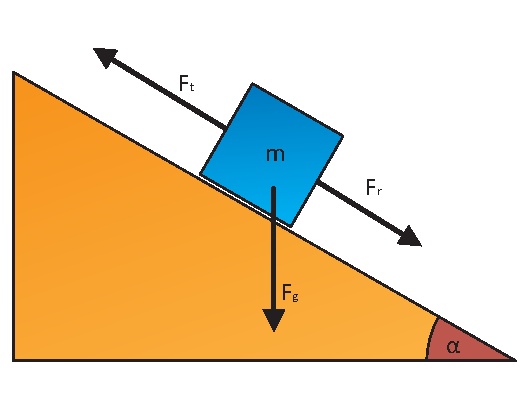
\includegraphics[height=4cm]{Newton-Pente}
\nextcol
	\[
		\left.\frac{\sum F_t - \sum R_r - F_g}{\sum m}\:\middle|F_g = m \cdot g \cdot \sin\alpha
		\right.
	\]
	\par\vspace{0.5em}
	\framenote{$\alpha = \tan^{-1}(\text{pente {\tiny en \%}})$}
\end{twocols}
\par\vspace{1em}
Système de poulies \\
\begin{twocols}[0.5][0.5]
	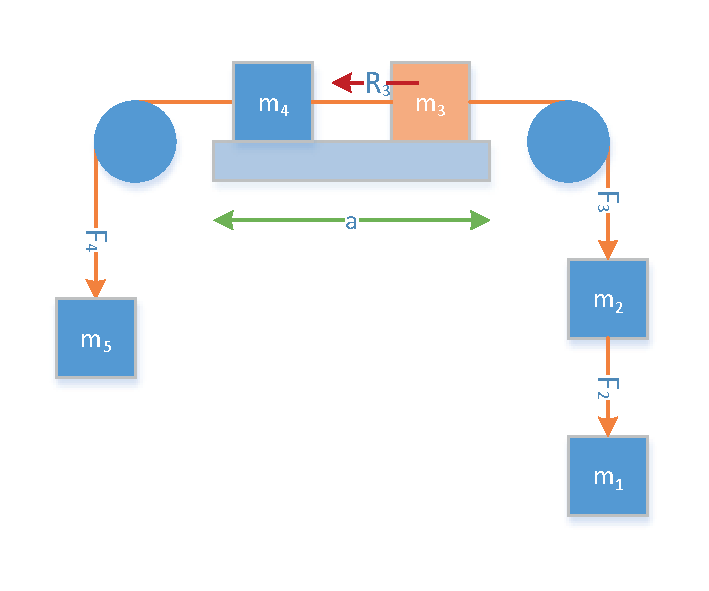
\includegraphics[width=1\textwidth]{Newton-Poulies}
\nextcol
	\begin{align*}
		a &= \frac{\sum F_n - \sum R_n}{\sum m_n} \\
		  &= \frac{g\cdot(m_1+m_2-m_5) - R_3}{|m_1|+|m_2|+|m_3|+|m_4|+|m_5|} \\
	\end{align*}
	\par\vspace{0.2em}
	Variables \\
	\begin{align*}
		F_n &= m_n \cdot g \\
		R_n &= \text{Résistance sur la masse $n$} \\
	\end{align*}
	\par\vspace{0.2em}
	\framenote{
		$F_n$ est nulle si l'objet n'est pas en suspension (ex $m_4$) \\
		Les masses qui ne sont pas en suspension et qui n'exercent pas de frottent sont tout de même comptées dans la somme des masses ($\sum m_n$)
	}

\end{twocols}
Forces de retenue et de traction \\
\begin{twocols}[0.5][0.5]
	\includegraphics[width=1\textwidth]{Newton-Traction}
\nextcol

	\begin{align*}
		F_t - F_g - F_r &= \sum m \cdot a \\
			F_g &= \sum m \cdot g \cdot \sin \alpha
	\end{align*}

	\framenote{La somme des masses est dépendant du sous-système choisi.}

\end{twocols}

\newpage

\subsection{Gravitation Universelle}

	\begin{figure*}[h]
		\centering
		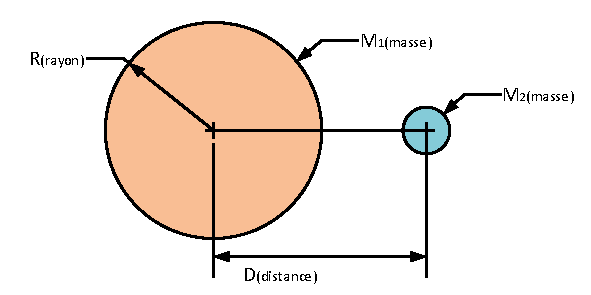
\includegraphics{Newton-Gravitation-1Planete}
	\end{figure*}

\begin{mdframed}[leftmargin=2em, rightmargin=2em]
	\frametitle{Loi de la Gravitation universelle}
	Deux corps quelconques s'attirent de manière proportionelle à leur masse et inversément proportionnelle au carré de leur distance. \\
	\par\hspace{0.5em}
	\begin{twocols}[0.3][0.3]
		\[F_G = G\cdot\frac{m_1 \cdot m_2}{d^2}\]
		\nextcol
		\begin{vardef}
			\item{$F_G$}{Force de gravitation [N]}
			\item{$G$}{Gravitation universelle [$N/m^2/kg$]}
					  & $6.67 \times 10^-11$ \\
			\item{$m_i$}{Masse [Kg]}
			\item{$d$}{Distance entre des corps [Km]}
		\end{vardef}
	\end{twocols}
\end{mdframed}
\par\hspace{1em}

\subsubsection*{Gravitation d'un corps}

\begin{figure*}[h]
	\centering
	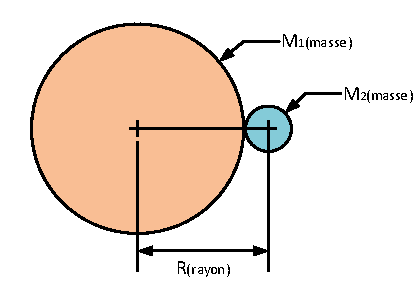
\includegraphics{Newton-Gravitation-Attraction}
\end{figure*}
Cette loi peut être dérivée lorsqu'un objet est suffisamment proche d'un corps de masse et taille beaucoup plus importantes. Le corps plus petit devient donc insignifiant.

	\[F_G = G\cdot\frac{m}{r^2}\]

\subsubsection*{Attraction entre deux champs de gravité}
\begin{figure*}[h]
	\centering
	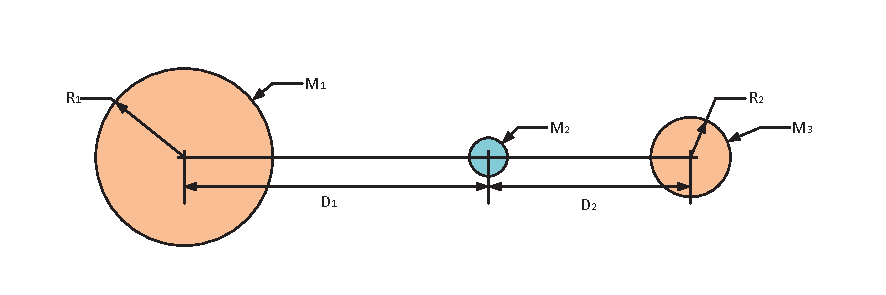
\includegraphics{Newton-Gravitation-2Planetes}
\end{figure*}
Une autre dérivation de cette loi peut s'appliquer lorsqu'un objet est soumis à deux champs de gravité distincts. Cette dérivation permet d'obtenir la direction et la vitesse avec laquel le corps au milieu se dirige.

	\[\left\{
		\begin{aligned}
			F &= G \cdot \left(\frac{m_1 \cdot m_2}{d_1\,^2} - \frac{m_3 \cdot m_2}{d_2\,^2}\right)\\
			F &= m_2 \cdot a\\
		\end{aligned}
	\right.\]

\subsubsection*{Équilibre d'attraction}
Lorsque l'objet se trouve à l'équilibre, l'accélération vaut 0. La formule peut donc être modifiée.

	\[\frac{m_1 \cdot m_2}{d_1\,^2} = \frac{m_3 \cdot m_2}{d_2\,^2}\]

\subsubsection*{Rapport des distances et des masses}
	\[\frac{d_1\,^2}{d_2\, ^2} = \frac{m_1}{m_3}\]

\newpage

\subsection{Mise en orbite}

\begin{figure*}[h]
	\centering
	\includegraphics[width=0.5\textwidth]{Newton-OrbiteGeostationnaire}
\end{figure*}

\begin{mdframed}
	Pour qu'un objet soit en orbite géosynchrone la force de gravité doit être égale à la force centripète.
	\[F_g = F_c\]
	\[\omega = \frac{\text{Angle parcouru [rad]}}{\text{Temps [s]}}\]

	\textbf{Generalisation} \\
	\begin{twocols}
		\begin{align*}
			G\cdot\frac{M_p\cdot M_o}{d^2} &= M_o \cdot \omega^2 \cdot d \\
			G \cdot M_p &= \omega^2 \cdot d^3 \\
			d &= r_p + alt \\
		\end{align*}

	\nextcol

		\begin{vardef}
			\item{$M_p$}{Masse de la planète [Kg]}
			\item{$M_o$}{Masse de l'objet [Kg]}
			\item{$d$}{Distance entre les corps [m]}
			\item{$r_p$}{Rayon de la planète [m]}
			\item{$alt$}{Altitude [m]}
		\end{vardef}

	\end{twocols}
	\\ \framenote{$\omega$ est equivalent a celui de la planète en orbite dans le cas d'une orbite géosynchrone}
\end{mdframed}

\vspace{1em}

\begin{mdframed}
	\frametitle{Nombre de passages au dessus d'un point pour une période donnée}

	\begin{twocols}
		\begin{align*}
			%%\omega_p \cdot n &= \omega_o \\[1em]
			\omega_0 &= \frac{2 \pi \cdot (n \pm 1)}{t} \\
			&= \omega_p \cdot (n \pm 1) & \text{(1)} \\
		\end{align*}
	\nextcol
		\begin{vardef}
			\item{$\omega_o$}{Vitsees angulaire de l'objet [rad/s]}
			\item{$\omega_p$}{$\omega$ de la planète [rad/s]}
			\item{$n$}{Nombre de tours}
			\item{$t$}{Temps [s]}
		\end{vardef}
		\\[1em]
		Sens identiques: $n+1$ \\
		Sens contraires: $n-1$ \\
		\framenote{(1) Passage sur un point}
	\end{twocols}
\end{mdframed}


\newpage

\section{Statique}
La statique est l'étude des forces sur un système à l'équilibre, la somme de ses forces est donc nulle.

	\[\sum \vec{F} = 0\]

Les forces sont considérées comme des vecteurs est s'additionnenet donc comme tels.

\subsection{Moment de Force}
Lorsqu'une force est appliquée sur un corps attaché à un axe de rotation, cette force produit un moment de force dont l'effet est propotionnel à la distance par rapport au centre de rotation et est mitigé par l'angle en fonction du corps.
\par\hspace{1em}

\begin{figure*}[h]
	\centering
	\includegraphics{Statique-Moments}
\end{figure*}
\begin{mdframed}[leftmargin=2em, rightmargin=2em]
	\begin{twocols}[0.5][0.5]
	\[
		\left\{
			\begin{aligned}
			F_\perp &= F \cdot \sin \alpha \\
			M &= F_\perp \cdot d \\
			\end{aligned}
		\right.
	\]

	\[\sum M = 0\]
	\nextcol
	\begin{vardef}
		\item{$M$}{Moment de force}
		\item{$F_\perp$}{Force perpendiculaire [N]}
		\item{$F$}{Force [N]}
		\item{$\alpha$}{Angle de la force [deg]}
	\end{vardef}
	\end{twocols}
\end{mdframed}

\newpage

\subsection{Système de forces}

\begin{figure*}[h]
	\centering
	\includegraphics{Statique-Axes}
\end{figure*}

\begin{mdframed}
	\frametitle{Equilibre}
	\begin{twocols}
		\[\left\{
		\begin{aligned}
			R_x &= \sum F_n \cdot \cos \alpha_n \\
			R_y &= \sum F_n \cdot \sin \alpha_n \\
		\end{aligned}
	\right.\]
	\nextcol
		\begin{vardef}
			\item{$R$}{Force résultante}
			\item{$F_n$}{Force en jeu}
		\end{vardef}
	\end{twocols}
	
\end{mdframed}

\newpage

\subsection{Centre de gravité}

\newcommand\fcount[1]{\text{nombre de}\left(#1\right)}

\begin{figure*}[h]
	\centering
	\includegraphics{Statique-CentreGravite}
\end{figure*}

\begin{twocols}[0.4][0.6]
	\begin{align*}
		m &= S \cdot d & \text{(1)} \\[1em]
		p &= \sum m \\[1em]
		G_x &= \frac{\sum\left(m_n \cdot x_n\right)}{p} \\[1em]
		G_y &= \frac{\sum\left(m_n \cdot y_n\right)}{p} \\
	\end{align*}
\nextcol
	\begin{vardef}
		\item{$m$}{Masse [Kg]}
		\item{$S$}{Surface [$m^2$]}
		\item{$d$}{Masse superficique [$Kg/m^2$]}
		\item{$p$}{Masse du système [Kg]}
		\item{$G_x\;\text{et}\;G_y$}{Coordonnée du centre de gravité [m]}
	\end{vardef}
	\par\vspace{0.5em}
	\framenote{(1) Le calcul $m = S \cdot d$ n'est pas applicable dans toutes les situations.}
\end{twocols}

\newpage

\section{Energie \& Puissance}

\subsection{Energie mécanique}

\subsubsection*{Travail de force}
\begin{figure*}[h]
	\centering
	\includegraphics[width=0.3\textwidth]{Mecanique-Generalite}
\end{figure*}
\begin{twocols}[0.5][0.5]
	\begin{align*}
		W &= F \cdot \ell \\
		  &= F_\parallel \cdot \ell \\
		  &= F \cdot \sin \alpha \cdot \ell \\
		  &= F \cdot \cos \beta \cdot \ell \\
	\end{align*}
\nextcol
	\begin{vardef}
		\item{$W$}{Travail de force [J]}
		\item{$F$}{Force [N]}
		\item{$\ell$}{Distance [m]}
		\item{$\alpha \: \beta$}{Angle [Deg]}
	\end{vardef}
\end{twocols}

\textbf{Formules dérivées}

\begin{figure*}[h]
	\centering
	\includegraphics[width=0.3\textwidth]{Mecanique-Travail}
\end{figure*}
Tavail de force sur une pente \\
\begin{twocols}[0.5][0.5]
	\begin{align*}
		h &= \sin \alpha \cdot d \\
		W &= h \cdot m \cdot g \\
	\end{align*}
\nextcol
	\begin{vardef}
		\item{$h$}{Dénivelé [m]}
		\item{$d$}{Distance [m]}
		\item{$m$}{Masse du corps [kg]}
	\end{vardef}
\end{twocols}

\newpage

\subsection{Energie Cynétique \& Potentielle}

\newcommand\ex[1]{E_{#1}}
\newcommand\ecin{\ex{\text{cin}}}
\newcommand\ecinx[1]{\ex{\text{cin}_{#1}}}
\newcommand\epot{\ex{\text{pot}}}
\newcommand\epotx[1]{\ex{\text{pot}_{#1}}}
\newcommand\sumw[1]{\sum W_{#1}}

\begin{mdframed}
	\frametitle{Théorème de l'énergie Cynétique}
	\begin{twocols}[0.4][0.6]
		\begin{align*}
			\ecinx{T} &= \frac{1}{2} \cdot m \cdot v^2 \\
			\sumw{AB} &= \ecinx{B} - \ecinx{A} \\
		\end{align*}
	\nextcol
		\begin{vardef}
			\item{$\ecinx{T}$}{Energie cinetique de translation [J]}
			\item{$m$}{Masse [N]}
			\item{$\sumw{AB}$}{Energie cynétique [N]}
		\end{vardef}
	\end{twocols}

\end{mdframed}
\vspace{1em}
\begin{mdframed}
	\frametitle{Energie Potentielle}
	\begin{twocols}[0.4][0.6]
		\begin{align*}
			\epotx{G} &= m_o \cdot g \cdot h \\
			\epotx{G} &= -G \cdot m_p \cdot m_o \cdot \frac{1}{\Delta h} & \text{(1)} \\
		\end{align*}
	\nextcol
		\begin{vardef}
			\item{$\epotx{G}$}{Energie potentielle de gravitation [J]}
			\item{$m_o$}{Masse objet [Kg]}
			\item{$m_p$}{Masse planète [Kg]}
			\item{$\Delta h$}{Diff. d'altitude [m]}
		\end{vardef}

		\framenote{(1) voir: Intégrations}

	\end{twocols}

\end{mdframed}

%% Formule WTF
%% \frametitle{Force de frottement \& décélération} \\
%% \begin{twocols}[0.5][0.5]
%% 	\begin{align*}
%% 		\Delta\ecinx{AB} &= - f \cdot d_f & \text{\itshape à plat} \\
%% 		&= m \cdot g \cdot d - f \cdot d_f & \text{\itshape en pente} \\
%% 	\end{align*}
%% \nextcol
%% 	\begin{vardef}
%% 		\item{$d$}{Distance [m]}
%% 		\item{$d_f$}{Distance d'arrêt [m]}
%% 		\item{$f$}{Force de frottement [N]}
%% 	\end{vardef}
%% \end{twocols}
\vspace{1em}
\frametitle{Différence de potentiel} \\
\[\Delta\epotx{AB} = \epotx{B} + \epotx{A}\]

%% Formule WTF
%% \frametitle{Objet en déplacement} \\
%% \[
%% 	\Delta\ecinx{AB} = \Delta\epotx{AB} + \ew{AB}
%% \]
\vspace{1em}
\frametitle{Intégrations}
\begin{align*}
	F(h) &= G \cdot \frac{m_p \cdot m_o}{h^2} \\
	\epotx{G} &= \integrate[h]{F(h)} \\
	\Delta\epotx{AB} &= \integratediff[h]{A}{B}{F(h)} \\
\end{align*}

\newpage

\subsection{Puissance}

\begin{mdframed}
	\frametitle{Théorème}

	\begin{twocols}
		\begin{align*}
			P &= \frac{E}{t} \\
			  &= \frac{F \cdot d}{t} \\
			  &= F \cdot v \\[1em]
		\end{align*}
	\nextcol
		\begin{vardef}
			\item{$P$}{Puissance [J/s = W(atts)]}
			\item{$E$}{Energie [J]}
			\item{$t$}{Temps [s]}
			\item{$F$}{Force [N]}
			\item{$v$}{Vitesse [m/s]}
		\end{vardef}
	\end{twocols}
\end{mdframed}
\vspace{1em}
\begin{mdframed}
	\frametitle{Rendement}
	\begin{align*}
		\text{Rendement} &= \frac{E_\text{Utile}}{E_\text{Fournie}} = \frac{P_\text{Utile}}{P_\text{Fournie}} \\[1em]
		\text{Perte} &= E_\text{Fournie} - E_\text{Utile} \\
		&= P_\text{Fournie} - P_\text{Utile} \\
	\end{align*}

\end{mdframed}

\newpage

\section{Sonique}

\subsection{Intensité et Décibels}
\begin{twocols}
	\begin{align*}
		\beta &= 10 \cdot \log_{10}\left(\frac{I}{I_0}\right) \\
	\end{align*}
\nextcol
	\begin{vardef}
		\item{$\beta$}{Décibels [db]}
		\item{$I$}{Intensité [$W/m^2$]}
		\item{$I_0$}{Seuil d'audition ($10^{-12}$) [$W/m^2$]}
	\end{vardef}
\end{twocols}

\subsection{Relations avec la pression}
\begin{twocols}
		\begin{align*}
		I &= \frac{(\Delta p)^2}{2 \cdot \rho \cdot V_\text{son}} \\
		\beta &= 20 \cdot \log_{20}\left(\frac{\Delta p}{\Delta p_0}\right) \\
	\end{align*}
\nextcol
	\begin{vardef}
		\item{$\Delta p$}{Amplitude (différence) de pression [Pa]}
		\item{$\rho$}{Masse volumique du milieu [$kg/m^3$]}
		\item{$V_\text{son}$}{Vitesse du son (dans l'air: 344 [m/s])}
		\item{$\beta$}{Décibels [db]}
		\item{$I$}{Intensité [$W/m^2$]}
	\end{vardef}
\end{twocols}

\subsubsection*{Autre formules}
\begin{twocols}
	\begin{align*}
		\frac{I_2}{I_1} &= 10^{\frac{\displaystyle \beta_2-\beta_1}{10}} \\
		\Delta\beta &= 10 \cdot \log_{10}(\Delta n)
	\end{align*}
\nextcol
	\begin{vardef}
		\item{$\Delta\beta$}{Diffèrence de décibels}
		\item{$\Delta n$}{Nombre de sources supplémentaires}
	\end{vardef}
\end{twocols}

\subsection{Dispersion sans amortissement}
\begin{figure*}[h]
	\centering
	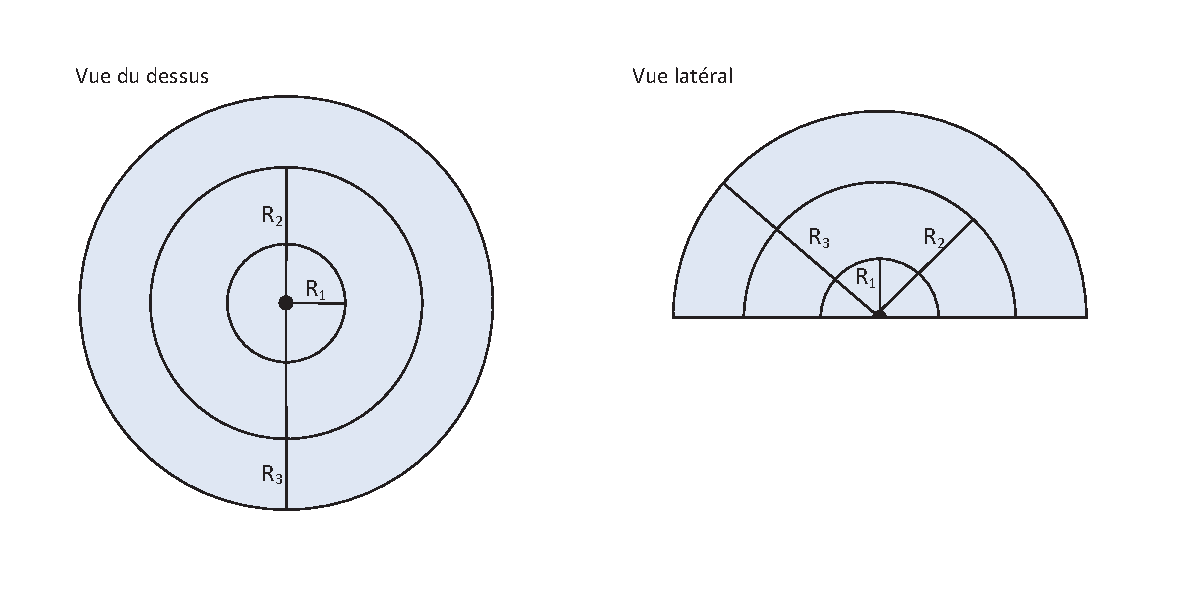
\includegraphics[width=0.75\textwidth]{Sonique-Dispersion}
\end{figure*}

\begin{twocols}[0.5][0.5]
	\begin{align*}
		I_1 \cdot S_1 &= I_2 \cdot S_2 \\
		I_1 \cdot {r_1}^2 &= I_2 \cdot {r_2}^2	\\[1em]
		\frac{I_2}{I_1} &= \frac{S_1}{S_2} \\
		\frac{I_2}{I_1} &= \left(\frac{r_1}{r_2}\right)^2 \\
	\end{align*}
\nextcol
	\begin{vardef}
		\item{$I_n$}{Intensité [$W/m^2$]}
		\item{$S_s$}{Surface de dispersion [$m^2$]}
		\item{$r_n$}{Rayon de dispersion [m]}
	\end{vardef}
\end{twocols}
\section{Transfert de chaleur}

\begin{mdframed}
	\frametitle{Théorème}
	\begin{twocols}
		\begin{align*}
			\sum Q &= 0 \\[1em]
			Q_n &= m \cdot c \cdot \Delta\theta & \text{Ch. température} \\
			&= m \cdot L & \text{Ch. état} \\
		\end{align*}
	\nextcol
		\begin{vardef}
			\item{$Q_n$}{Energie [J]}
			\item{$\Delta\theta$}{Diff. de temperature [°C]}
			\item{$m$}{Masse [kg]}
			\item{$c$}{Chaleur specifique [J/kg/°C]}
			\item{$L$}{Chaleur latente de transformation [J/kg]}
		\end{vardef}
	\end{twocols}
\end{mdframed}

\subsection{Formules dérivées}

\frametitle{Equilibre de temperature}
Pour obtenir un équilibre de température, il faut que l'énergie cédée par les corps chauds soit absorbée par les corps froids.
\[\sum \text{énergie cédée} = \sum \text{énergie absorbée}\]

\frametitle{Source d'énergie externe}
Lorsqu'un système est alimenté par une source d'énergie externe, il l'absorbe entièrement excepté les éventuelles pertes.
\[\sum E_\text{reçue} - \sum E_\text{perte} = \sum Q\]

\frametitle{Développement}
\begin{vardef}
	\item{$T_1$}{Température initiale [°C]}
	\item{$T_2$}{Température finale [°C]}
\end{vardef}
\begin{align*}
	\Delta Q &= m \cdot (c_\text{glace} \cdot (0-\theta_1) + L_\text{fusion} + c_\text{eau} \cdot (\theta_2 - 0))
\end{align*}

\newpage

\tableofcontents
\vspace{2em}
\frametitle{\large Contributeurs} \\
\begin{description}[style=nextline]
	\item[Jeremy David] sti34a 2013, \texttt{http://github.com/ltouroumov}, \texttt{ltouroumov@gmail.com}
	\item[Kevin Wenger] sti34a 2013, \texttt{http://github.com/sudei}
	\item[Timothée Moulin] sti34a 2013, \texttt{http://github.com/tehem}
	\item[Vincent Kobel] sti34a 2013
\end{description}
%% {\large\bfseries Correcteurs} \\
%% \begin{description}[style=nextline]
%% 	\item[Olivier Pittet] Enseignant CPNV
%% \end{description}

%----------------------------------------------------------------------------------------

\end{document}
